\documentclass[11pt]{beamer}

\usetheme{metropolis}


\usepackage[utf8]{inputenc}
\usepackage{ucs}
\usepackage[brazil]{babel}
\usepackage[T1]{fontenc}
\usepackage{amsmath}
\usepackage{amsfonts}
\usepackage{amssymb}
\usepackage{graphicx}
\usepackage{subfigure}
\usepackage{ragged2e}
\usepackage{fancybox}
\usepackage{tikz}



\usepackage{color}
\usepackage{fancyhdr}
\pagestyle{fancy}
\usepackage{xcolor}
\usepackage{xwatermark}

\title{CAPITULO 4 \\ Testando hipóteses}
\author{Márcia}
\institute{Instituto de Matemática e Estatística \\Faculdade de Estatística}
\date{2019}

\begin{document}

\maketitle

%%%%%%%%%%%%%%%%%%%%%%%%%%%%%%%%%%%%

\section{Testando hipóteses}

%%%%%%%%%%%%%%%%%%%%%%%%%%%%%%%%%%%%

\subsection{Quadro de testes de hipóteses}

%%%%%%%%%%%%%%%%%%%%%%%%%%%%%%%%%%%%

\begin{frame}
\frametitle{Lembre-se de quando...}

Experiência de discriminação de gênero:

{\small
\begin{tabular}{ll  cc c} 
  		&				& \multicolumn{2}{c}{\textit{Promotion}} \\
\cline{3-4}
							&			& Promovido	& Não Promovido	& Total	\\
\cline{2-5}
\multirow{2}{*}{\textit{Gênero	}}	&Masculino 		& 21	 	& 3		& 24 	\\
							&Feminino		& 14	 	& 10 	 	& 24 \\
\cline{2-5}
							&Total		& 35		& 13		& 48 \\
\end{tabular}
}

\pause

\[ \hat{p}_{homens} = 21 / 24 \approx 0.88 \]
\[ \hat{p}_{mulheres} = 14 / 24 \approx 0.58 \]

\pause

Explicações possíveis:
\begin{itemize}
\item Promoção e gênero são \hl{independentes}, não há discriminação de gênero, a diferença observada em proporções é simplesmente devido ao acaso. $\rightarrow$ \orange{nulo} - {\small (nada está acontecendo)}
\item Promoção e gênero são \hl{dependentes}, há discriminação de gênero, a diferença observada nas proporções não se deve ao acaso. $\rightarrow$ \orange{alternativa} - {\small (algo está acontecendo)}

\end{itemize}

\end{frame}

%%%%%%%%%%%%%%%%%%%%%%%%%%%%%%%%%%%%

\begin{frame}
\frametitle{Resultado}

\begin{center}
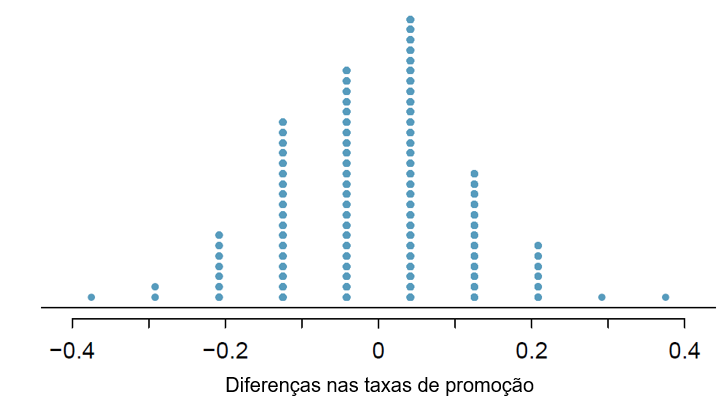
\includegraphics[width=0.75\textwidth]{discRandDotPlot.pdf}
\end{center}

\pause

Como era bastante improvável obter resultados como os dados reais ou algo mais extremo nas simulações (promoções masculinas sendo 30 \% ou mais superiores às promoções femininas), decidimos rejeitar a hipótese nula em favor da alternativa.

\end{frame}

%%%%%%%%%%%%%%%%%%%%%%%%%%%%%%%%%%%%

\begin{frame}
\frametitle{Recapitulação: estrutura de teste de hipóteses}

\begin{itemize}
\item Começamos com uma \hl{hipótese nula ($ H_0 $)} que representa o status quo.
\pause
\item Também temos uma hipótese \hl{alternative ($ H_A $)} que representa nossa questão de pesquisa, ou seja, o que estamos testando.
\pause
\item Realizamos um teste de hipóteses sob o pressuposto de que a hipótese nula é verdadeira, seja através de simulação ou métodos tradicionais baseados no teorema do limite central (chegando próximo ...).
\pause
\item Se os resultados do teste sugerirem que os dados não fornecem evidências convincentes para a hipótese alternativa, nós nos ateremos à hipótese nula. Se o fizerem, rejeitamos a hipótese nula em favor da alternativa.
\end{itemize}
\pause
Introduziremos formalmente a estrutura de testes de hipóteses usando um exemplo para testar uma afirmação sobre uma média populacional.

\end{frame}

%%%%%%%%%%%%%%%%%%%%%%%%%%%%%%%%%%%%

\subsection{Testando hipóteses usando intervalos de confiança} 

%%%%%%%%%%%%%%%%%%%%%%%%%%%%%%%%%%%%

\begin{frame}
\frametitle{Testando hipóteses usando intervalos de confiança}

\dq{Anteriormente, calculamos um intervalo de confiança de 95 \% para o número médio de relacionamentos exclusivos em que os estudantes universitários estavam (2,7, 3,7). Com base nesse intervalo de confiança, esses dados confirmam a hipótese de que os estudantes universitários, em média, têm mais de três relacionamentos exclusivos.}

\pause

\begin{itemize}

\item As hipóteses associadas são:
\begin{itemize}
\item[$H_0$:] $\mu = 3$: Os estudantes universitários têm estado em três relacionamentos exclusivos, em média
\item[$H_A$:] $\mu > 3$: Os estudantes universitários têm mais de 3 relacionamentos exclusivos, em média
\end{itemize}

\pause

\item Como o valor nulo é incluído no intervalo, não rejeitamos a hipótese nula em favor da alternativa.

\pause

\item Esta é uma abordagem rápida e suja para testes de hipóteses. No entanto, não nos diz a probabilidade de certos resultados sob a hipótese nula, ou seja, o valor p, com base no qual podemos tomar uma decisão sobre as hipóteses.

\end{itemize}

\end{frame}

%%%%%%%%%%%%%%%%%%%%%%%%%%%%%%%%%%%%

\begin{frame}
\frametitle{Número de pedidos de faculdade}

\dq{{\small Uma pesquisa semelhante perguntou quantas faculdades os alunos aplicaram e 206 alunos responderam a essa pergunta. Esta amostra rendeu uma média de 9,7 aplicações universitárias com um desvio padrão de 7. O site do College Board afirma que os orientadores recomendam que os alunos se inscrevam em aproximadamente 8 faculdades. Esses dados fornecem evidências convincentes de que o número médio de colégios aos quais os alunos da Duke se candidatam é \emph{superior} do que o recomendado?}}

\vfill

\ct{\webURL{http://www.collegeboard.com/student/apply/the-application/151680.html}}

\end{frame}

%%%%%%%%%%%%%%%%%%%%%%%%%%%%%%%%%%

\begin{frame}
\frametitle{Definindo as hipóteses}

\begin{itemize}

\item O \hl{parâmetro de interesse} é o número médio de escolas aplicadas por \underline{todos} estudantes da Duke.

\pause

\item Pode haver duas explicações por que nossa média de amostra é maior do que as 8 escolas recomendadas.
\begin{itemize}
\item A verdadeira média populacional é diferente.
\item A média real da população é 8, e a diferença entre a média real da população e a média da amostra é simplesmente devido à variabilidade natural da amostragem.
\end{itemize}

\pause

\item Começamos com a suposição de que o número médio de estudantes em que os alunos da Duke se candidatam é 8 (como recomendado)
\[ \mathhl{H_0:}~\mu = 8 \]

\pause

\item Testamos a alegação de que o número médio de estudantes em que os alunos da Duke se candidatam é maior que 8
\[ \mathhl{H_A:}~\mu > 8 \]

\end{itemize}

\end{frame}

%%%%%%%%%%%%%%%%%%%%%%%%%%%%%%%%%%%

\subsection{Condições para inferência}

%%%%%%%%%%%%%%%%%%%%%%%%%%%%%%%%%%%

\begin{frame}
\frametitle{Número de candidaturas universitárias - condições}

\pq{Qual das seguintes opções é \emph{não} uma condição que precisa ser atendida para prosseguir com este teste de hipótese?}

\begin{enumerate}[(a)]
\item Os alunos da amostra devem ser independentes uns dos outros em relação a quantas faculdades se candidataram.
\item A amostragem deveria ter sido feita aleatoriamente.
\item O tamanho da amostra deve ser menor que 10 \% da população de todos os alunos da Duke.
\solnMult{ Deve haver pelo menos 10 sucessos e 10 falhas na amostra.}
\item A distribuição do número de colégios aplicados pelos alunos não deve ser extremamente assimétrica.
\end{enumerate}

\end{frame}

%%%%%%%%%%%%%%%%%%%%%%%%%%%%%%%%%%

\subsection{Teste formal usando valores de p}

%%%%%%%%%%%%%%%%%%%%%%%%%%%%%%%%%%%%

\begin{frame}
\frametitle{Estatística de teste}

Para avaliar se a média da amostra observada é incomum para a distribuição de amostragem hipotética, determinamos quantos erros-padrão estão fora do nulo, o que também é chamado de \hl{estatística de teste}.


\pause

\twocol{0.55}{0.45}{
\begin{center}
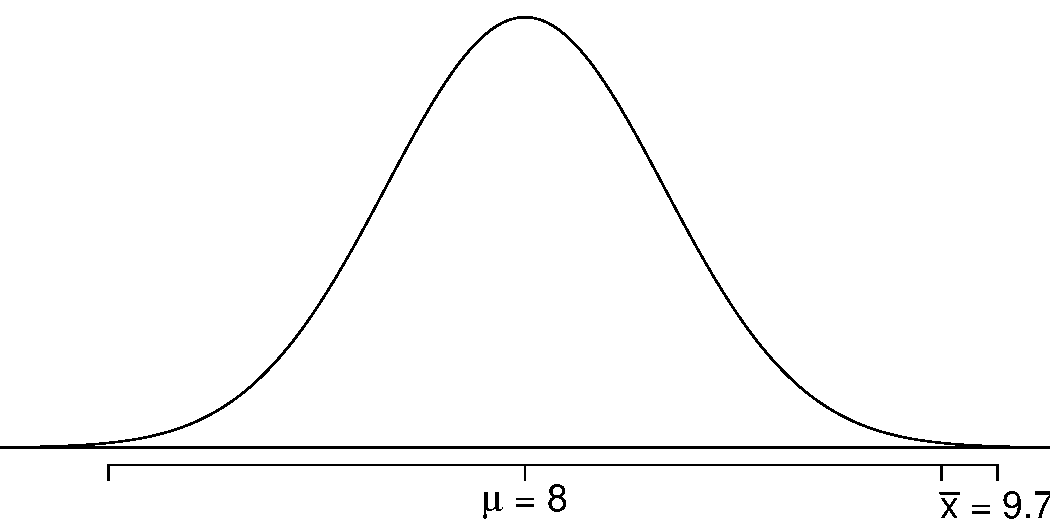
\includegraphics[width=\textwidth]{app_z.pdf}
\end{center}
\pause
\[ \bar{x} \sim N \pr{ \mu = 8, SE = \frac{7}{\sqrt{206}} = 0.5 } \]
\pause
\[ Z = \frac{9.7 - 8}{0.5} = 3.4 \]
}
{
\pause
\dq{A média da amostra é de 3,4 erros padrão longe do valor hipotético. Isso é considerado excepcionalmente alto? Ou seja, é o resultado \hl{estatisticamente significante}?}
\pause
\soln{Sim, e podemos quantificar o quão incomum é usar um valor-p.}
}

\end{frame}

%%%%%%%%%%%%%%%%%%%%%%%%%%%%%%%%%%%

\begin{frame}
\frametitle{valores de p}

\begin{itemize}

\item Em seguida, usamos essa estatística de teste para calcular o valor de \hl {p-valor}, a probabilidade de observar dados pelo menos tão favoráveis à hipótese alternativa quanto nosso conjunto de dados atual, se a hipótese nula fosse verdadeira.


\pause

\item Se o valor p for \hl {baixo} (menor que o nível de significância, $ \alpha $, que normalmente é de 5 \%), dizemos que seria muito improvável observar os dados se a hipótese nula fosse verdadeira, e daí \hl {rejeitar $ H_0 $}.

\pause

\item Se o valor p for \hl {high} (maior que $ \alpha $), dizemos que é provável observar os dados mesmo se a hipótese nula fosse verdadeira e, portanto, \hl {não rejeitar $ H_0 $}.

\end{itemize}

\end{frame}

%%%%%%%%%%%%%%%%%%%%%%%%%%%%%%%%%%%%

\begin{frame}
\frametitle{Número de inscrições em faculdades - valor p}

\hl{p-valor:} probabilidade de observar dados pelo menos tão favoráveis a $ H_A $ como nosso conjunto de dados atual (uma média de amostra maior que 9,7), se de fato $ H_0 $ fossem verdadeiros (a média real da população era 8).


\begin{center}
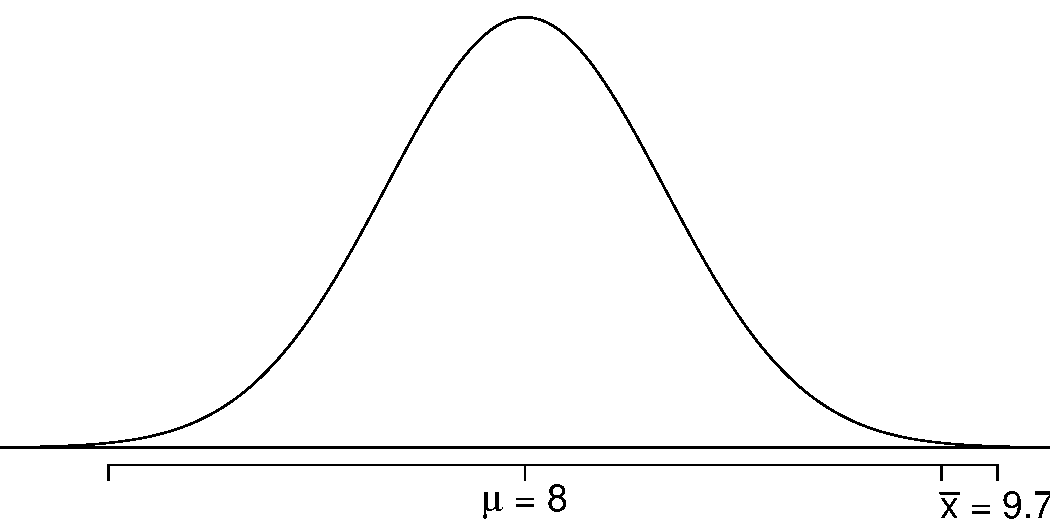
\includegraphics[width=0.55\textwidth]{app_pval_gr.pdf}
\end{center}

\pause

\[ P(\bar{x} > 9.7~|~\mu = 8) = P(Z > 3.4) = 0.0003 \]

\end{frame}

%%%%%%%%%%%%%%%%%%%%%%%%%%%%%%%%%%

\begin{frame}
\frametitle{Número de inscrições em faculdades - tomada de decisão}

\begin{itemize}

\item p-value = 0.0003

\pause

\begin{itemize}
\item Se a média real do número de estudantes em que os alunos da Duke se candidataram é 8, há apenas 0,03 \% de chance de observar uma amostra aleatória de 206 alunos da Duke que, em média, aplicam-se a 9,7 ou mais escolas.

\pause
\item Esta é uma probabilidade muito baixa para nós pensarmos que uma média amostral de 9,7 ou mais escolas provavelmente acontecerá por acaso.
\end{itemize}

\pause
\item Como o valor p é \orange {baixa} (menor que 5 \%), nós \orange {rejeitamos $ H_0 $}.

\pause
\item Os dados fornecem evidências convincentes de que os alunos da Duke se aplicam a mais de 8 escolas em média.

\pause
\item A diferença entre o valor nulo de 8 escolas e a média amostral observada de 9,7 escolas é \laranja {não por acaso} ou variabilidade amostral.

\end{itemize}

\end{frame}

%%%%%%%%%%%%%%%%%%%%%%%%%%%%%%%%%%%%

\begin{frame}
\frametitle{}

\pq{{\footnotesize Uma pesquisa da National Sleep Foundation descobriu que os estudantes universitários têm em média 7 horas de sono por noite. Uma amostra de 169 estudantes universitários que fizeram uma aula de estatística introdutória rendeu uma média de 6,88 horas, com um desvio padrão de 0,94 horas. Supondo que esta seja uma amostra aleatória representativa de todos os estudantes universitários {\scriptsize \textit{(com um pouco de fé?)}}, um teste de hipótese foi realizado para avaliar se os estudantes universitários em média sono \emph{menos que} 7 horas por noite. O valor p para este teste de hipótese é 0,0485. Qual das seguintes opções está correta?}}

\begin{enumerate}[(a)]
\item Deixar de rejeitar $ H_0 $, os dados fornecem evidências convincentes de que os estudantes universitários dormem em média menos de 7 horas.
\solnMult{ Rejeitar $ H_0 $, os dados fornecem evidências convincentes de que os estudantes universitários dormem menos de 7 horas em média. }
\item Rejeitar $ H_0 $, os dados provam que os estudantes universitários dormem mais de 7 horas em média.
\item Deixar de rejeitar $ H_0 $, os dados não fornecem evidências convincentes de que os estudantes universitários dormem menos de 7 horas em média.
\item Rejeitar $ H_0 $, os dados fornecem evidências convincentes de que os estudantes universitários nesta amostra dormem menos de 7 horas em média.
\end{enumerate}

\end{frame}

%%%%%%%%%%%%%%%%%%%%%%%%%%%%%%%%%

\subsection{Teste de hipóteses de dois lados com valores de p}

%%%%%%%%%%%%%%%%%%%%%%%%%%%%%%%%%

\begin{frame}
\frametitle{Teste de hipóteses de dois lados com valores de p}

\begin{itemize}

\item Se a pergunta de pesquisa for "Os dados fornecem evidências convincentes de que a média de sono dos estudantes universitários por noite é \orange{diferente} que a média nacional? ", a hipótese alternativa seria diferente.
\begin{align*}
H_0&: \mu = 7 \\
H_A&: \mu \orange{~$\ne$~} 7
\end{align*}

\pause

\item Portanto, o valor p também mudaria:
\twocol{0.55}{0.45}
{
\begin{center}
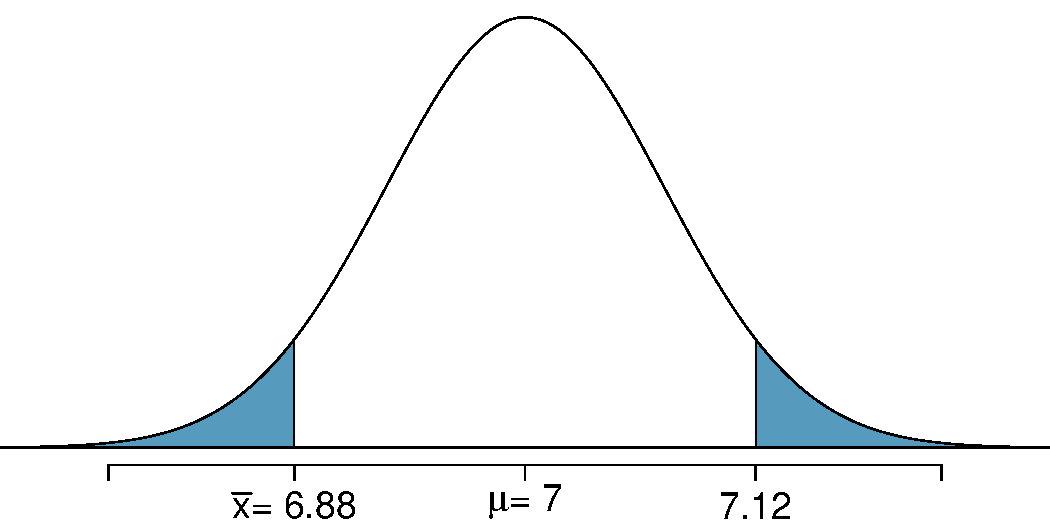
\includegraphics[width=\textwidth]{sleep_pval_ts.pdf}
\end{center}
}
{
valor-p \\
$= 0.0485 \times 2$ \\
$= 0.097$
}

\end{itemize}

\end{frame}

%%%%%%%%%%%%%%%%%%%%%%%%%%%%%%%%%%%%

\subsection{Erros de decisão}

%%%%%%%%%%%%%%%%%%%%%%%%%%%%%%%%%%%%

\begin{frame}
\frametitle{Erros de decisão}

\begin{itemize}

\item Testes de hipóteses não são perfeitos.

\item No sistema judiciário, pessoas inocentes são às vezes erroneamente condenadas e os culpados às vezes andam livres.

\item Da mesma forma, podemos tomar uma decisão errada também nos testes de hipóteses estatísticas.

\item A diferença é que temos as ferramentas necessárias para quantificar a frequência com que cometemos erros nas estatísticas.

\end{itemize}

\end{frame}

%%%%%%%%%%%%%%%%%%%%%%%%%%%%%%%%%%%%

\begin{frame}
\frametitle{Erros de decisão (cont.)}

Existem duas hipóteses concorrentes: a nula e a alternativa. Em um teste de hipótese, tomamos uma decisão sobre o que pode ser verdade, mas nossa escolha pode estar incorreta. \\

\pause

\begin{center}
\begin{tabular}{l l | c c}
\multicolumn{2}{c}{} & \multicolumn{2}{c}{\textbf{Decisão}} \\
& & não rejeitar $H_0$ &  rejeitar $H_0$ \\
  \cline{2-4}
& $H_0$ verdadeiro & \onslide<3->{\green{$\checkmark$}} &  \onslide<5->{\orange{Erro tipo 1}} \\
\raisebox{1.5ex}{\textbf{Verdade}} & $H_A$ true & \onslide<6->{\orange{Erro tipo 2}} & \onslide<4->{\green{$\checkmark$}} \\
  \cline{2-4}
\end{tabular}
\end{center}

\begin{itemize}
\item \onslide<5->{Um \hl{erro tipo 1} está rejeitando a hipótese nula quando $ H_0 $ é verdadeiro.}

\item \onslide<6->{Um \hl {Erro tipo 2} não está conseguindo rejeitar a hipótese nula quando $ H_A $ é verdadeiro.}

\item \onslide<7->{Nós (quase) nunca sabemos se $ H_0 $ ou $ H_A $ é verdade, mas precisamos considerar todas as possibilidades.}

\end{itemize}

\end{frame}

%%%%%%%%%%%%%%%%%%%%%%%%%%%%%%%%%%%%

\begin{frame}
\frametitle{Teste de Hipótese como um julgamento}

Se pensarmos novamente em um teste de hipótese como um processo criminal, então faz sentido enquadrar o veredicto em termos das hipóteses nula e alternativa:
\begin{align*}
H_0&:\text{ Réu é inocente} \\
H_A&:\text{ Réu é culpado}
\end{align*}

Qual tipo de erro está sendo cometido nas seguintes circunstâncias?

\begin{itemize}
\item Declarando o réu inocente quando eles são realmente culpados
\soln{\only<2->{\begin{center}\hl{Erro tipo 2}\end{center}}}
\item Declarando o réu culpado quando eles são realmente inocentes
\soln{\only<3->{\begin{center}\hl{Erro tipo 1}\end{center}}}
\end{itemize}

\only<4->{Qual erro você acha que é o pior erro para fazer?}
\only<5>{\begin{center}{\footnotesize ``melhor que dez pessoas culpadas escapar do que aquele inocente sofrem''\\ -- William Blackstone}\end{center}}
\end{frame}

%%%%%%%%%%%%%%%%%%%%%%%%%%%%%%%%%%%%

\begin{frame}
\frametitle{Taxa de erro de tipo 1}

\begin{itemize}

\item Como regra geral, rejeitamos $ H_0 $ quando o valor p é menor que 0,05, ou seja, usamos um \hl {nível de significância} de 0,05, \mathhl{\alpha = 0.05}.

\pause

\item Isso significa que, nos casos em que $ H_0 $ é realmente verdadeiro, não queremos rejeitá-lo incorretamente mais de 5 \% desses horários. 

\pause

\item Em outras palavras, ao usar um nível de significância de 5 \%, há cerca de 5 \% de chance de gerar um erro de Tipo 1 se a hipótese nula for verdadeira.
\[ \mathhl{ P(\text{Erro tipo 1 | $H_0$ Verdade}) = \alpha } \]

\pause

\item É por isso que preferimos valores pequenos de$\alpha$ -- aumentando $\alpha$ aumenta a taxa de erro do tipo 1.

\end{itemize}

\end{frame}

%%%%%%%%%%%%%%%%%%%%%%%%%%%%%%%%%%%%

\subsection{Escolhendo um nível de significância}

%%%%%%%%%%%%%%%%%%%%%%%%%%%%%%%%%%%%

\begin{frame}
\frametitle{Escolhendo um nível de significância}

\begin{itemize}

\item Escolher um nível de significância para um teste é importante em muitos contextos, e o nível tradicional é de 0,05. No entanto, geralmente é útil ajustar o nível de significância com base no aplicativo. 

\item Podemos selecionar um nível menor ou maior que 0,05, dependendo das consequências de quaisquer conclusões obtidas no teste.

\item Se um Erro Tipo 1 for perigoso ou especialmente caro, devemos escolher um nível de significância pequeno (por exemplo, 0,01). Sob este cenário, queremos ser muito cautelosos ao rejeitar a hipótese nula, então exigimos evidências muito fortes favorecendo $ H_A $ antes de rejeitarmos $ H_0 $.

\item Se um Erro Tipo 2 for relativamente mais perigoso ou muito mais dispendioso do que um Erro Tipo 1, então devemos escolher um nível de significância mais alto (por exemplo, 0,10). Aqui, queremos ter cautela ao não rejeitar $ H_0 $ quando o valor nulo for realmente falso.

\end{itemize}

\end{frame}

%%%%%%%%%%%%%%%%%%%%%%%%%%%%%%%%%%%%

\subsection{Recap}

%%%%%%%%%%%%%%%%%%%%%%%%%%%%%%%%%%%%

\begin{frame}

\vfill

\textit{próximas paginas serão fornecidos como um breve resumo dos testes de hipóteses..}

\vfill

\end{frame}

%%%%%%%%%%%%%%%%%%%%%%%%%%%%%%%%%%%%

\begin{frame}
\frametitle{Recapitulação: estrutura de testes de hipóteses}

\begin{enumerate}

\item Defina as hipóteses.

\item Verifique as suposições e condições.

\item Calcule uma \hl {estatística de teste} e um valor p.

\item Tome uma decisão e interprete-a no contexto da questão de pesquisa.

\end{enumerate}

\end{frame}

%%%%%%%%%%%%%%%%%%%%%%%%%%%%%%%%%%%

\begin{frame}
\frametitle{Recapitulação: teste de hipóteses para uma média populacional}

\begin{enumerate}

\item Defina as hipóteses
\begin{itemize}
\item $H_0: \mu = null~value$
\item $H_A: \mu <$ ou $>$ ou $\ne null~value$
\end{itemize}

\item Calcular a estimativa pontual

\item Verifique as suposições e condições
\begin{itemize}
\item Independência: amostra / atribuição aleatória, condição de 10 \% quando amostragem sem substituição
\item Normalidade: população quase normal ou $ n \ge 30 $, sem assimetria extrema - ou use a distribuição t
\end{itemize}

\item Calcule uma \ hl {estatística de teste} e um valor p (desenhe uma figura!)
\[ Z = \frac{\bar{x} - \mu}{SE},~onde~SE = \frac{s}{\sqrt{n}} \]

\item Tome uma decisão e interprete-a no contexto
\begin{itemize}
\item Se o valor de p $ <\alpha $, rejeitar $ H_0 $, os dados fornecerão evidências de $ H_A $
\item Se o valor p $> \alpha $, não rejeitar $ H_0 $, os dados não fornecem evidência para $ H_A $
\end{itemize}

\end{enumerate}

\end{frame}

%%%%%%%%%%%%%%%%%%%%%%%%%%%%%%%%%%%%

\end{document}
